\documentclass[12pt]{report}
\usepackage[utf8]{inputenc}
\usepackage{graphicx}
\graphicspath{ {../images/} }
\usepackage{setspace}
\usepackage{sectsty}

% code snippets

\usepackage{listings}
\usepackage{color}

\definecolor{dkgreen}{rgb}{0,0.6,0}
\definecolor{gray}{rgb}{0.5,0.5,0.5}
\definecolor{mauve}{rgb}{0.58,0,0.82}

\lstset{frame=tb,
  language=Python,
  aboveskip=3mm,
  belowskip=3mm,
  showstringspaces=false,
  columns=flexible,
  basicstyle={\small\ttfamily},
  numbers=none,
  numberstyle=\tiny\color{gray},
  keywordstyle=\color{blue},
  commentstyle=\color{dkgreen},
  stringstyle=\color{mauve},
  breaklines=true,
  breakatwhitespace=true,
  tabsize=3
}

%

\chapterfont{\fontsize{20}{18}\selectfont \centering}

\title{
{Classifying Hindustani Indian Ragas with Convolutional Neural Networks}\\
{\large Pitzer College}\\
{
\includegraphics{university_1.png}}
}
\author{Rishov S. Chatterjee\\[1cm]{Advisor: Dr. Yan Li}}
\date{13 May 2019}
\begin{document}
\maketitle{}

\doublespacing
\setlength{\parindent}{1cm}

\begin{center}
  \textbf{\large Words of Acknowledgement}
\end{center}
I would like to exhibit words of gratitude to Dr. Yan Li for teaching me about data mining, machine learning, and database technologies to develop a thorough understanding required to do a thesis of this magnitude. I would also like to thank Dr. Michael Spezio at Scripps College for deepening my understanding of machine learning through its application with neural signals and sharing his wisdom about audio signal processing and words of advice about conducting end-to-end machine learning for any project. Also, I give many thanks to my advisor, Dr. Linus Yamane at Pitzer College for believing in my academic efforts through his constant support and communication with me. Finally, I want to thank my father, Dr. Samir Chatterjee at Claremont Graduate University for supporting me through every trial and tribulation during my undergraduate career.


\chapter*{\centering Introduction}
\doublespacing
\setlength{\parindent}{1cm}

\par

I have been exposed to Hindustani classical music ever since I was small. I was raised in an Indian household to immigrant parents and my mom is a vocalist and an exponent of Indian classical music. Indian classical music is categorized into two distinct forms: Hindustani and Carnatic, which are practiced in North and Southern India. Unlike western classical music, Indian classical music is very old form and typically doesn’t have clear structures but largely depends on the performers or instrument players own elaboration of a melody. Indian classical music is defined by two basic elements – it must follow a Raga (classical mode), and a specific rhythm, the Taal [1]. Most compositions follow a Raga and I have noticed that even experts sometimes have difficulty of telling which Raga a particular song or composition is based on. This is particularly challenging for novices or beginners. Being a data science major, I quickly became attracted to this problem of “Raga detection”. My intuition said that machine learning algorithms and techniques could help classify a composition into a main Raga on which it is based. Thus begins my journey to explore and hence this senior thesis. \par

I will mainly focus on North Indian form which is referred to as the Hindustani classical music. Compositions in Hindustani classical music also are based on a drone, i.e., a continual pitch that sounds throughout the concert, which is tonic [2]. This drone acts as a point of reference as the performer is expected to come back to this home base after a flight of improvisation. The variations and complexity in Hindustani music stems from its use of notes that comprise a Raga. There are seven main musical notes (also called swaras) – Sa, Re, Ga, Ma, Pa, Dha and Ni – along with five intermediate notes (flats and sharps) referred to as “vikrit swaras”. The seven notes are referred to as Shuddha and belongs to the saptak (a scale). The flat notes are called “komal” and the sharp notes are called “teevra”. A raga consists of at least five notes, and each raga provides the musician with a musical framework within which to improvise [3, 4 5]. The specific notes within a raga can be reordered and improvised by the musician. Ragas range from small ragas like Bahar and Shahana that are not much more than songs to big ragas like Malkauns, Darbari and Yaman, which have great scope for improvisation and for which performances can last over an hour. Each raga traditionally has an emotional significance and symbolic associations such as with season, time and mood [6].  The raga is considered a means in Indian musical tradition to evoke certain feelings in an audience. Hundreds of raga are recognized in the classical tradition, of which about 30 are common [7]. \par

The swaras in a raga can be played in three octaves, the first or lower octave starting from 130 Hz, then middle octave starting at 260 Hz; and upper octave from 520 Hz. The artists are allowed to improvise over the definitions of raga to create their own renditions. If you listen to two performance of the same raga, they may sound strikingly different to novice ears, though they still retain the rules and defining qualities of ragas. \par


\chapter*{\centering Indian Classical Ragas}
\doublespacing
\setlength{\parindent}{1cm}


\chapter*{\centering Librosa: Processing Musical Information in Python}
\doublespacing
\setlength{\parindent}{1cm}

The research field of music information retrieval (MIR) has been evolving rapidly. Taken broadly, it covers the area of musicology, digital signal processing, machine learning, information retrieval and library science. As digital music service platforms such as iTunes, Spotify and Pandora have grown, so has been the need for MIR tools which to date has been largely written by programmers as scripts using C++ or MATLAB. In recent years, interest has grown within the MIR community in using (scientific) Python as a viable alternative [ref]. LibROSA is a python package for music and audio analysis. It provides the building blocks necessary to create music information retrieval systems. Here I provide a brief introduction to basic ideas and elements in libROSA as I have used this package in conducting bulk of the work in my thesis.
\par
In general, librosa’s functions tend to expose all relevant parameters to the caller. While this provides a great deal of flexibility to expert users, it can be overwhelming to novice users who simply need a consistent interface to process audio files. To satisfy both needs, they define a set of general conventions and standardized default parameter values shared across many functions.
\par
An audio signal is represented as a one-dimensional numpy array, denoted as y throughout librosa. Typically the signal y is accompanied by the sampling rate (denoted sr) which denotes the frequency (in Hz) at which values of y are sampled. The duration of a signal (d) can then be computed by dividing the number of samples (y) by the sampling rate (sr): \par
\begin{center}
  $ d = \frac{y}{sr} $
\end{center}

\begin{lstlisting}
# duration_seconds.py
from librosa import load
import os
# Getting all mp3 files of raga Bhairav from dataset
fileList = os.listdir("data/Hindustani/mp3/Bhairav")
# Creating dictionary to store number of samples and sampling rate
sampleDict = {}
# y is number of samples, sr is sampling rate of the audio file
for file in fileList:
  y, sr = load(file)
  sampleDict[file].append(y)
  sampleDict[file].append(sr)
  # calculating signal duration
  duration = y / sr
  sampleDict[file].append(duration)
\end{lstlisting}

By default, when loading stereo audio files, the librosa.load() function down mixes to mono by averaging left- and right-channels, and then resamples the monophonic signal to the default rate $ sr=22050Hz $. Most audio analysis methods operate not at the native sampling rate of the signal, but over small frames of the signal which are spaced by a hop length (in samples). The default frame and hop lengths are set to 2048 and 512 samples, respectively. At the default sampling rate of 22050 Hz, this corresponds to overlapping frames of approximately 93ms spaced by 23ms. Frames are centered by default, so frame index t corresponds to the slice:

\begin{lstlisting}
  y[(t*hop_length - frame_length/2):(t*hop_length+frame_length/2)]
\end{lstlisting}

where boundary conditions are handled by reflection padding the input signal y. For analyses that do not use fixed-width frames (such as the constant-Q transform), the default hop length of 512 is retained to facilitate alignment of results.

\par

The majority of feature analyses implemented by librosa produce two-dimensional outputs stored as numpy.ndarray, e.g., S[f, t] might contain the energy within a particular frequency band f at frame index t. We follow the convention that the final dimension provides the index over time, e.g., S[:, 0],  S[:,1] access features at the first and second frames. Feature arrays are organized column-major (Fortran style) in memory, so that common access patterns benefit from cache locality. By default, all pitch-based analyses are assumed to be relative to a 12-bin equal-tempered chromatic scale with a reference tuning of A440 = 440.0 Hz. Pitch and pitch-class analyses are arranged such that the 0th bin corresponds to C for pitch class or C1 (32.7 Hz) for absolute pitch measurements.

\par
\begin{flushleft}
  \textbf{Core Functionality}
\end{flushleft}

The librosa.core submodule includes a range of commonly used functions. Broadly, core functionality falls into four categories: audio and time-series operations, spectrogram calculation, time and frequency conversion, and pitch operations [ref]. For convenience, all functions within the core submodule are aliased at the top level of the package hierarchy, e.g., ``librosa.core.load'' is aliased to ``librosa.load''.
\par
Audio and time-series operations include functions such as: reading audio from disk via the audioread package [ref], resampling a signal at a desired rate, stereo to mono conversion, time-domain bounded auto-correlation, and zero-crossing detection. Spectrogram operations include the short-time Fourier transform (stft), inverse STFT (istft), and instantaneous frequency spectrogram (ifgram) [Abe \space 95], which provide much of the core functionality for down-stream feature analysis. Additionally, an efficient constant-Q transform (cqt) implementation based upon the recursive down-sampling method of Schoerkhuber and Klapuri [ref] is provided, which produces logarithmically-spaced frequency representations suitable for pitch-based signal analysis. Finally, logamplitude provides a flexible and robust implementation of log-amplitude scaling, which can be used to avoid numerical underflow and set an adaptive noise floor when converting from linear amplitude. Since data may be represented in a variety of time or frequency units, a comprehensive set of convenience functions is provided to map between different time representations: seconds, frames, or samples; and frequency representations: hertz, constant-Q basis index, Fourier basis index, Mel basis index, MIDI note number, or note in scientific pitch notation. Finally, the core submodule provides functionality to estimate the dominant frequency of STFT bins via parabolic interpolation (piptrack) [Smith \space 11], and estimation of tuning deviation (incents) from the frequency reference A440. These functions allow pitch-based analyses (e.g., cqt) to dynamically adapt filter banks to match the global tuning offset of a particular audio signal.

\par
\begin{flushleft}
  \textbf{Spectral Features}
\end{flushleft}

Spectral representations are the distributions of energy over a set of frequencies which form the basis of many analysis techniques in MIR and digital signal processing in general. Librosa implements a variety of spectral representations, most of which are based upon the short \space time Fourier transform. The Mel frequency scale is commonly used to represent audio signals, as it provides a rough model of human frequency perception [ref]. Both a Mel-scale spectrogram and the commonly used Mel-frequency Cepstral Coefficients (MFCC) are provided. By default, Mel scales are defined to match the implementation provided by Slaney’s auditory toolbox [ref], but they can be made to match the Hidden Markov Model Toolkit (HTK). While Mel \space scaled representations are commonly used to capture timbral aspects of music, they provide poor resolution o pitches and pitch classes. Pitch class (or chroma) representations are often used to encode harmony while suppressing variations in octave height, loudness, or timbre. Two flexible chroma implementations are provided: one uses a fixed-window STFT analysis (chroma \_ stft) [ref] and the other uses variable-window constant-Q transform analysis (chroma\_cqt). An alternative representation of pitch and harmony can be obtained by the tonnetz function, which estimates tonal centroids as coordinates in a six-dimensional interval space using the method of Harte et \space al. [ref]. Figures 1,2,3, and 4 illustrate the difference between STFT, Mel spectrogram, chromagram, and Tonnetz representations.

\begin{flushleft}
  \textbf{Display}
\end{flushleft}

The display module provides simple interfaces to visually render audio data through matplotlib [ref]. The first function, display.waveplot simply renders the amplitude envelope of an audio signal y using matplotlib’s fill\_between function. For efficiency purposes, the signal is dynamically down-sampled.
\par
Mono signals are rendered symmetrically about the horizontal axis; stereo signals are rendered with the left-channel’s amplitude above the axis and the right-channel’s below. An example of waveplot is depicted in Figure 2 (top). The second function, display.specshow wraps matplotlib’s imshow function with default settings (origin and aspect) adapted to the expected defaults for visualizing spectrograms. Additionally, specshow dynamically selects appropriate colormaps (binary, sequential, or diverging) from the data type and range [ref]. Finally, specshow provides a variety of acoustically relevant axis labeling and scaling parameters. Examples of specshow output are displayed in Figures 1,2,3, and 4.

\begin{figure}
  \caption{Specshow Outputs for STFT, Mel Spectrogram, Chroma\_CQT, and Tonnetz Representations}
  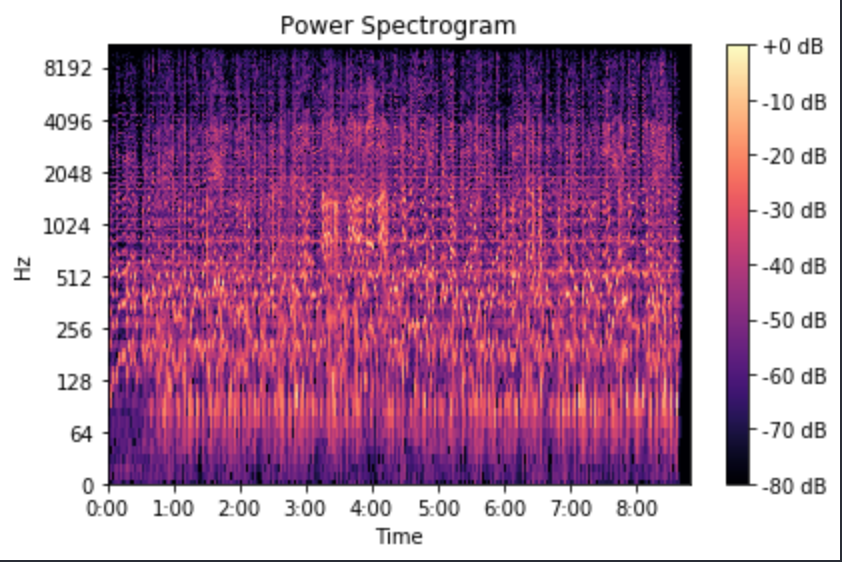
\includegraphics{stft-specgram.png}
\end{figure}
\begin{figure}
  \caption{Specshow Outputs for STFT, Mel Spectrogram, Chroma\_CQT, and Tonnetz Representations}
  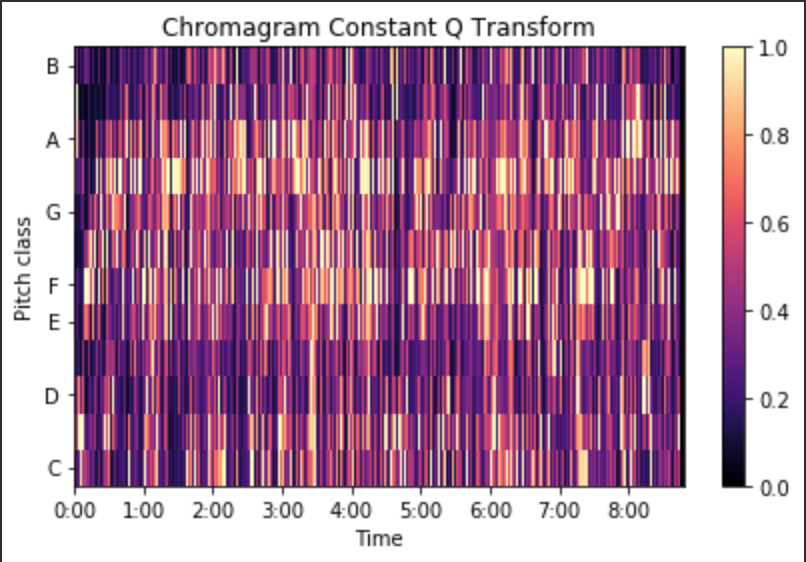
\includegraphics{chroma-cqt.png}
\end{figure}
\begin{figure}
  \caption{Specshow Outputs for STFT, Mel Spectrogram, Chroma\_CQT, and Tonnetz Representations}
  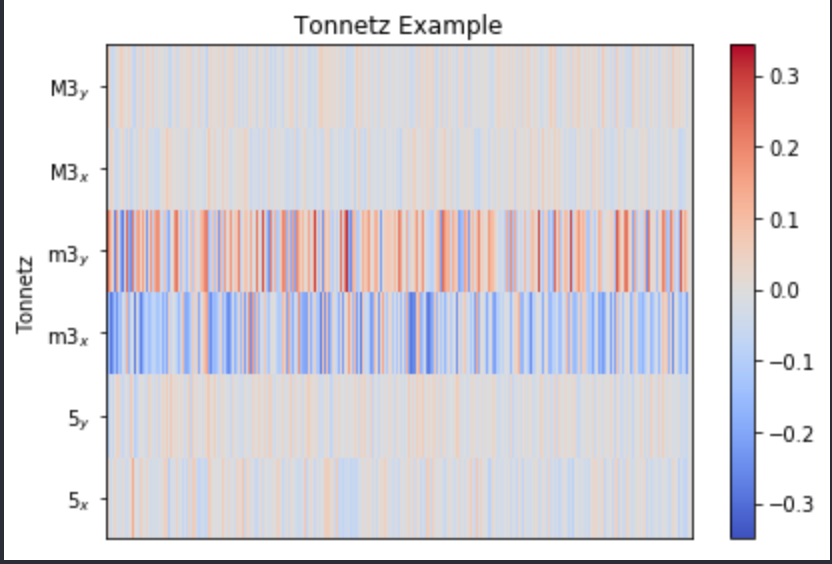
\includegraphics{tonnetz.png}
\end{figure}
\begin{figure}
  \caption{Specshow Outputs for STFT, Mel Spectrogram, Chroma\_CQT, and Tonnetz Representations}
  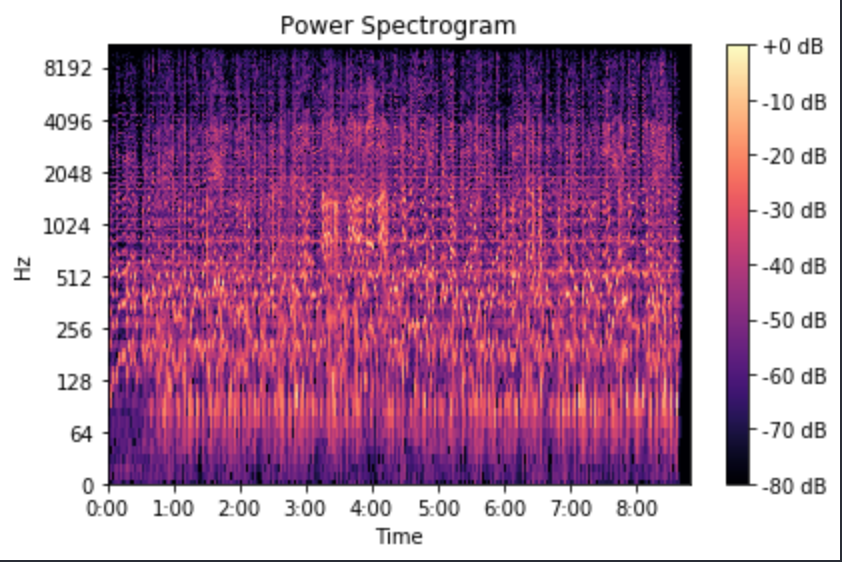
\includegraphics{stft-specgram.png}
\end{figure}


\chapter*{\centering Background and Related Work}
\doublespacing
\setlength{\parindent}{1cm}

Scholars and researchers have used different mechanisms to identify ragas. In a system called Tansen, Pandey (Pandey, Mishra, and Ipe, 2003) created a system in which a raga is automatically identified based on Hidden markov model. Pendekar (Pendekar et. al. 2013) were able to identify a raga by segmentation of audio signal via spectral flux and thereby identifying raga by using its pitch frequency. Certain other researchers such as Chelpa (Chelpa, 1991) proposed a fuzzy set theory for generation of alap patterns. Sreedhar et. al. (Sreedhar and Gita, 2009), created a database of ragas and used the scale of the raga performance as a similarity metric using nearest neighbors algorithms. Within a scale, notes are matched with the existing sets of notes in the ragas in the database. The closest raga in the database is given as output for the test raga.
\par
Tzanetakis (Tzanetakis and Cook, 2002) has also proposed various schemes in the English music classification based on their moods and styles of the performer as well as songs genre classification. Clustering is suggested as the classifier (Vaska, 2015). Sentiment analysis of movie review based on naïve Bayes and genetic algorithm is suggested in Govindarajan (Govindarajan, 2013). Since this methodology depends on the likelihood it can be connected to a wide assortment of spaces and results can be utilized as a part of numerous ways (Sharma, 2018). Shetty et. al., (Shetty and Achary, 2009) has identified raga based upon arohana-avorahana pattern on different ragas using neural network technique.
\par
In a 2015 paper (Sharma and Bali, 2015), Sharma and Bali compared several ML classifiers to dataset of music labeled by 4 ragas: Des, Bhupali, Yaman and Todi. The audio performances are converted into .wav extension and chroma features are extracted using MIR toolbox in Matlab. A hop factor of 0.025 second is selected which gives 4719 frames. Then they were able to extract the Vadi swara, also known as the king swara whose magnitude and pitch are relatively greater than notes (swaras). Then they used the WEKA tool which includes a comprehensive collection of machine learning algorithms. The dataset of different ragas is classified using machine learning classifiers in WEKA. Classifiers they used are Random Forest, C4.5, Bayesian network and K-star. After performing comparison of classifiers on ragas, they observed that K-star gives the largest accuracy of 93.38\%, on dataset of ragas followed by the random forest with 92.64\%.
\par
In another work, Kumar et. al. (Kumar et. al. 2014), proposed a method to identify the ragas of an Indian Carnatic music signal. They discuss why this problem is hard due to i) the absence of a fixed frequency for a note, ii) relative scale of notes, iii) oscillations around the note, and iv) improvisations. In this work, they framed the raga classification problem in a non-linear SVM framework using a combination of two kernels that represent the similarities of a music signal using two different features pitch-class profile and n-gram distribution of notes. This differs from the previous pitch-class profile based approaches where the temporal information of notes is ignored. They evaluated the proposed approach on their own raga dataset and CompMusic dataset (CompMusic, 2019) and show an improvement of 10.19\% by combining the information from two features relevant to Indian Carnatic music.
\par
In a recent article, Ale Koretzky (Koretzky, 2019) provides valuable guidance on music signal processing that is helpful for the work that I have to do. Ale addresses the problem of how can we extract vocals out of a mixed track? This is formally known as Audio Source Separation. When we look at a audio source file (,m3 or ,wav), we are visualizing a waveform in the time domain. All we have access to are the amplitude values of the signal over time. While it is possible to extract features like envelopes, RMS values, zero-crossing rate etc., but these features aren’t strong discriminators. To extract vocal content from a mix, we must somehow expose the structure of human speech. This is where the Short-Time Fourier Transform (STFT) comes to our rescue.
\par
\begin{figure}
  \caption{Short Term Fourier Transform of Vocal Audio Sample}
  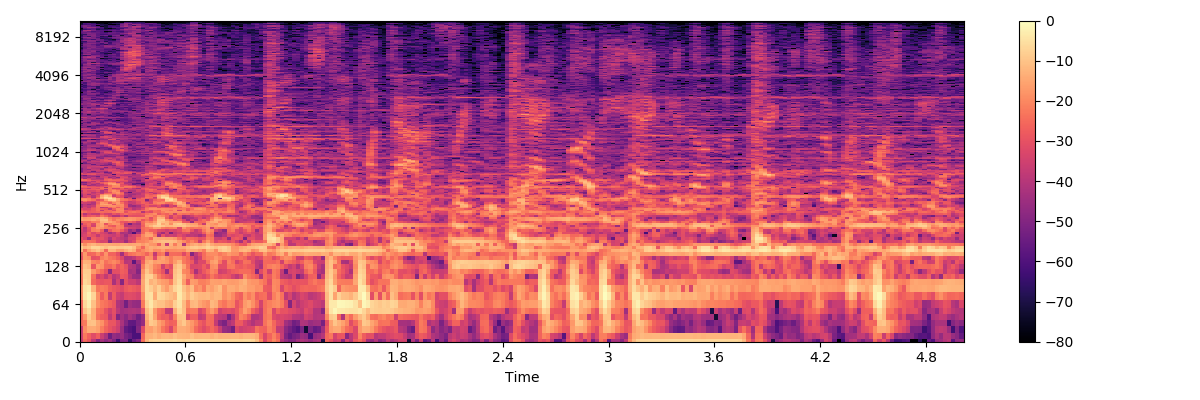
\includegraphics[width=150mm]{vocal-stft.png}
\end{figure}
What the STFT plot shows us are:
\begin{enumerate}[i]
  \item a fundamental frequency (f0) determined by the frequency of the vibration of our vocal cords.
  \par
  The figure below shows Ariana (Koretzky, 2019) is singing in the 300-500 Hz range.
  \item A number of harmonics above f0 following some shape or pattern
  \item no unvoiced speech, which includes consonants like `t', `p,', `k', `s', breaths, etc. \par
  They manifest as short bursts in the high frequency.
\end{enumerate}

The basic idea now is to figure out some sort of mask that when applied (element-wise multiplication) to the magnitude STFT mix gives us an approximate reconstruction pf the magnitude of STFT of the vocals. If this idea works, then we can begin to look at Convolutional Neural Networks (CNN) and what they have been able to achieve on images. Since STFT exhibits spatial patterns (in the time versus frequency space), CNNs should be able to learn from.

\par

Using CNNs on spectral information extracted from librosa to learn patterns has not been explored much in prior work. This is the approach I am going to take in the thesis. My research question becomes:  \par

\textbf{Can CNNs learn and classify ragas based on spectral features represented within chromagrams?}

Before answering this question, it is first important to review what a convolutional neural network is as well as its underlying mechanics for recognizing images in the next chapter.


\chapter*{\centering Methodology}
\doublespacing
\setlength{\parindent}{1cm}

\begin{flushleft}
  \textbf{Design of an End to End Raga Data Pipeline}
\end{flushleft}

For this thesis, I had to think of a way to get a dataset of images that I can then use for training a convolutional neural network architecture. In order to go about this process, I decided to first understand how I will look at getting audio files in which I know the raga associated with each file. I will then convert each audio file into a chromagram with a short term Fourier transform in order to get spectral information as well as differences in pitch over the duration of the audio file. In order to get multiple chromagrams for each audio file, I decided to generate a chromagram for each minute of the audio file's duration. To make this possible, I had to use an advanced I\/O feature in Librosa known as blockwise reading. Since Librosa did not have blockwise reading on its own, I had to make use of another library in tandem with Librosa for making this possible. The name of this second library is known as PySoundFile which is a Python wrapper for SoundFile which makes blockwise-reading possible as well as a functionality for metadata information regarding any input audio file as long as it in a .wav format. This premise presented a challenge for me as it required a conversion from a compressed .mp3 format of medium quality into .wav to input files as arguments into SoundFile's functional interface.

\begin{flushleft}
  \textbf{Converting from MP3 to WAV}
\end{flushleft}

Since MP3 files are a compressed, digital format of audio data based on the bit rate measured in kilobits per second [ref], I first decided to look into those values surrounding the mp3 quality from my initial dataset of mp3 files. Since the dataset is based on medium-quality mp3 files, I deduced that the bit rate, x, will be a range bounded between $ (128 < x < 320) $ kbps depending on the extracted mp3 files from the dataset's architect. Since I do not have control over the variance in bit rates nor time to generate a uniform dataset of mp3 files, I decided to go straight into the conversion of the mp3 format to the wav format. In order to do this, I made use of a Python module known as scikit-sound. Scikit-sound [ref] is a very useful utility as it makes it possible to read compressed audio file formats and encode them into wav format by making use of a third party utility known as FFMPEG. FFMPEG has a sampling algorithm to scale various audio formats based on the type of audio conversion that needs to be done. For the case of scaling from mp3 to wav in which the file size is much greater, FFMPEG samples at a standard sampling rate based on a default encoding from mp3 to wav. The encoding is not readily observable by the end user. FFMPEG is considered as the engine within scikit-sound's Sound class. From the software point of view, a simple instantiation of the Sound class with the input being the mp3 file will automatically read a wav file of the same file name while disregarding the .mp3 extension. Fortunately, FFMPEG is available across many operating systems and so I was able to install it using the Homebrew package manager within my Macbook. The uniform sampling rate from FFMPEG becomes a huge convenience when going into block reading which will be discussed more specifically in the next section.

\begin{lstlisting}
  # An instance of Scikit-Sound's Sound Class
  # Python 3.6+
  from sksound.sounds import Sound
  import os

  fileList = os.listdir("/path to raga audio files in mp3 format")
  # dictionary to store each instantiated response
  fileDict = {}
  # iterating through every file
  for file in fileList:
    fileDict[file] = Sound(f"path/{file}")
\end{lstlisting}

Each wav file will be in the same directory as the path which contains the mp3 files. To alleviate this challenge, I created a directory structure as follows:

\begin{figure}
  \caption{Directory Structure for Audio Files}
  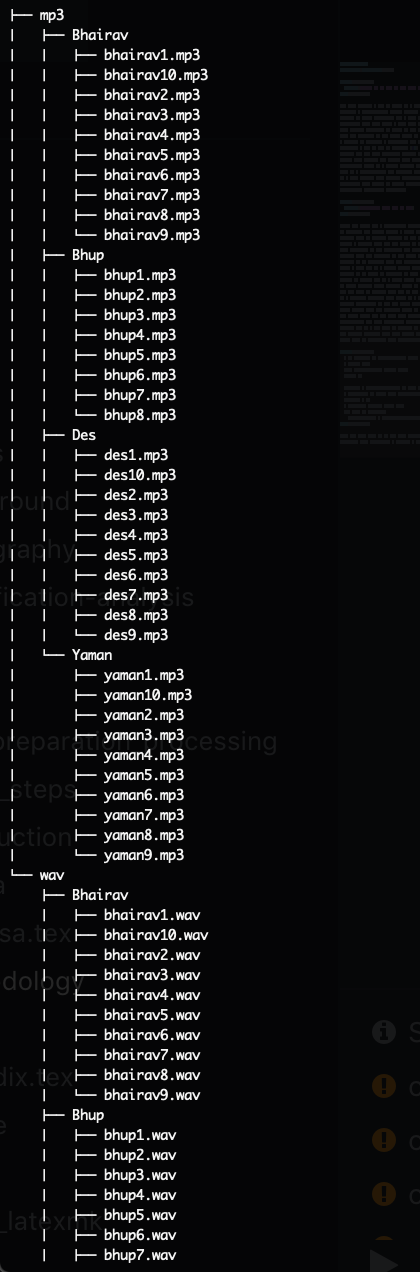
\includegraphics{audio-directory.png}
  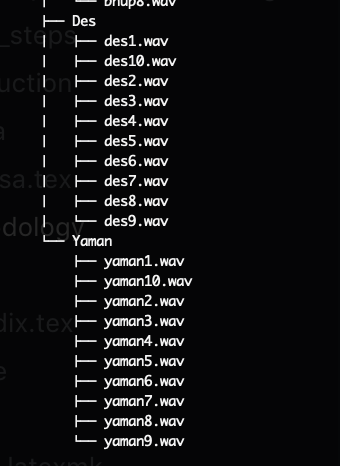
\includegraphics{audio-directory2.png}
\end{figure}

Once the wav files finished generating for each specific raag, I ran the following bash commands in my Terminal to move all the wav files into the wav directory.

\begin{lstlisting}
  cd data/Hindustani/mp3/Bhairav && mv *.wav ../../wav/Bhairav
  cd data/Hindustani/mp3/Bhup && mv *.wav ../../wav/Bhup
  cd data/Hindustani/mp3/Des && mv *.wav ../../wav/Des
  cd data/Hindustani/mp3/Yaman && mv *.wav ../../wav/Yaman
\end{lstlisting}

I also want to note that in order to perform proper version controlling of all my code commits, I tracked all mp3 and wav files using git-lfs so they would be known to Git and my GitHub repository as large files and will therefore be written to GitHub upon pushing commits with a higher file writing rate than that of normally pushed files.

\begin{flushleft}
  \textbf{Block-Wise Reading with PySoundFile}
\end{flushleft}

As mentioned before, I wanted to read the audio files as blocks of a certain size in order to generate stft-chromagrams for each minute in every audio file. To calculate the block size, b, I used the following equation in which sr refers to the sampling rate per second and n refers to the number of seconds:

$$ b = sr * n $$

To get the specific sampling rate which FFMPEG used for sampling, I used an attribute of PySoundFile.

\begin{lstlisting}
  # importing PySoundFile
  import soundfile as sf
  import os
  bhairavList = os.listdir("data/Hindustani/wav/Bhairav")
  for file in bhairavList:
    rate = sf.info(f"data/Hindustani/wav/Bhairav/{file}").samplerate
    print(rate)
\end{lstlisting}

The sampling rate that FFMPEG used for converting from mp3 to wav for the audio files corresponding to each raga is 44100 Hz. This means that in order to get a chromagram for each minute in the audio file, n would have to be equal to 60 since there are 60 seconds in a minute.

My uniform blocksize computes to:

$$ b = 44100 * 60 = 2646000 $$

After getting this value, reading in audio files into Librosa in tandem with PySoundFile's functionality became a very trivial matter.

\begin{lstlisting}
import numpy as np
# importing soundfile and librosa
!pip install pysoundfile
import soundfile as sf
from librosa.feature import chroma_stft
from librosa.display import specshow
import matplotlib.pyplot as plt
# Bhairav Block Wise Reading

## Bhairav 1

block_gen = sf.blocks('data/Hindustani/wav/Bhairav/bhairav1.wav', blocksize=2646000)
rate = sf.info("data/Hindustani/wav/Bhairav/bhairav1.wav").samplerate
info = sf.info("data/Hindustani/wav/Bhairav/bhairav1.wav")
print(info)
chromas = []

for bl in block_gen:
    y = np.mean(bl, axis=1)
    chromas.append(chroma_stft(y, sr=rate))

len(chromas)
for j, chroma in enumerate(chromas):
    specshow(chroma, x_axis="time", y_axis="chroma", vmin=0, vmax=1)
    plt.title(f"Chromagram of Bhairav1_{j}")
    plt.savefig(f"data/chroma_files/bhairav-chromas/bhairav1/bhairav1_{j}.png")
\end{lstlisting}

The above script allowed me to automate the generation of stft-chromagrams for every one minute block in the first audio recording of raga Bhairav. After thinking about the iterative process, I managed to build a more powerful automation script that would be able to generate chromagrams for every block for every audio file for a specific raga.  An example of this process is shown below to generate stft-chromagrams for all the audio files of the dataset I used for raga, Bhup.

\begin{lstlisting}
import os
import numpy as np
import soundfile as sf
from librosa.feature import chroma_stft
from librosa.display import specshow
import matplotlib.pyplot as plt

bhup_files = os.listdir("data/Hindustani/wav/Bhup")
print(bhup_files)

# Generating directories to denote each bhup audio file an iterative path

for h,i in enumerate(bhup_files):
    os.system(f"mkdir data/chroma_files/bhup-chromas/bhup{h+1}")

# Creating an empty dictionary to store

chroma_dict = {}

for j in range(len(bhup_files)):

    # building blocks for each file pertaining to the Bhup raga

    rate = sf.info(f"data/Hindustani/wav/Bhup/bhup{j+1}.wav").samplerate
    block_gen = sf.blocks(f"data/Hindustani/wav/Bhup/bhup{j+1}.wav", blocksize=rate*60)
    chroma_dict[f"bhup{j+1}"] = []

    # Computing the chroma_stft for every block in each Bhup audio file

    for bl in block_gen:
        y = np.mean(bl, axis=1)
        chroma_dict[f"bhup{j+1}"].append(chroma_stft(y, sr=rate))

    # Visualizing and saving the stft-chromagram for every block for every Bhup audio file
    # naming convention: bhup[file enumeration]_[block number]

    for k, chroma in enumerate(chroma_dict[f"bhup{j+1}"]):
        specshow(chroma, x_axis="time", y_axis="chroma", vmin=0, vmax=1)
        plt.title(f"Chromagram of Bhup{j+1}_{k+1}")
        plt.savefig(f"data/chroma_files/bhup-chromas/bhup{j+1}/bhup{j+1}_{k+1}.png")
\end{lstlisting}

The figure below illustrates the file structure for the generated chromagrams as png files.

\begin{figure}
  \caption{File Structure for Stored Bhup and Bhairav STFT-Chromagram Images}
  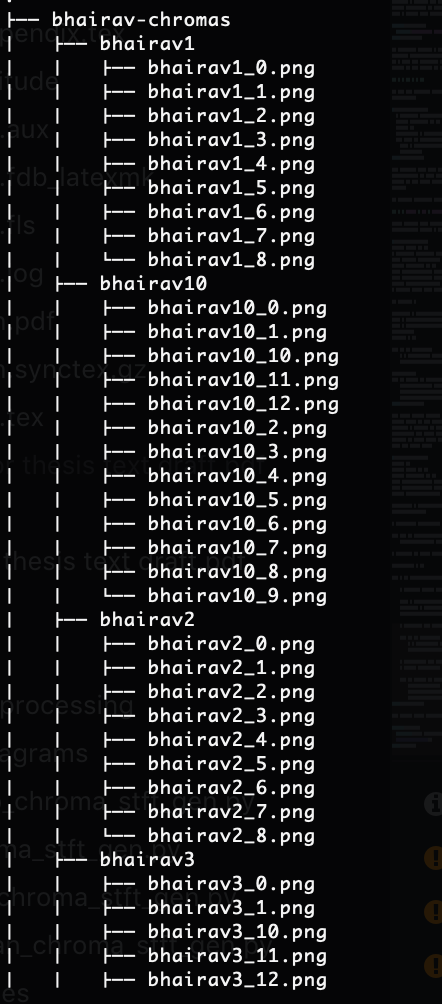
\includegraphics{bhairav-chroma-tree.png}
  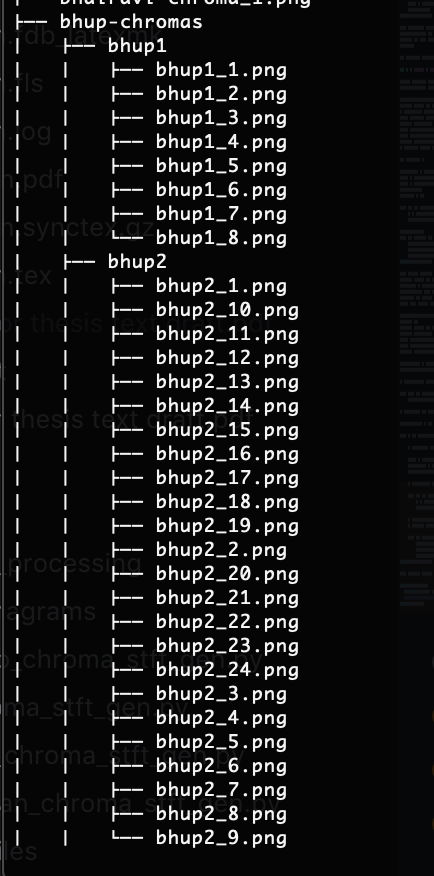
\includegraphics{bhup-chroma-tree.png}
\end{figure}

\begin{flushleft}
  \textbf{Data Preparation for CNN Training}
\end{flushleft}

In order to have the images ready for a machine learning experiment with a convolutional neural network, I first needed to generate a csv file of labels corresponding to the raga of each recording. Since I had an original file structure comprising of all the images of all the ragas, building up labels for all the files became very trivial and the ragas were all in
alphabetical order. The script below shows the process I used in pandas to build the miml\_labels\_2 csv file.

\begin{lstlisting}
import pandas as pd
import os

# Empty dictionary

columnDict = {}

# Getting all image files in one Python list

fileList = os.listdir("data")
print(len(fileList))

columnDict['file_name'] = fileList

print(columnDict)

# Empty list to store labels

labels = []

# Range values calculated beforehand

for i in range(202):
  labels.append("bhairav")

for i in range(183):
  labels.append("bhup")

for i in range(137):
  labels.append("des")

for i in range(258):
  labels.append("yaman")

print(len(labels))

# Generating second column to store labels

columnDict['raga'] = labels

# Converting from a dictionary to a Pandas DataFrame

df = pd.DataFrame.from_dict(columnDict)

# Saving DataFrame as a Comma Separated Value (csv) file

df.to_csv("csv/miml_labels_2.csv")

\end{lstlisting}

\begin{flushleft}
  \textbf{CNN Preprocessing and Training with Tensorflow 2.0 and Keras on Google Colab}
\end{flushleft}

Now that I had my CSV file and image data, I moved over from my local environment to Google Colaboratory in order to make use of a free tier graphics processing unit (GPU) optimized for neural network training with ease offered by the Google Compute Engine (GCE) with a memory allocation of 12 GB RAM.
\par
In order to make this transition simple, I created another GitHub repository which contains 780 stft-chromagram images as well as the csv file pertaining to labels that correspond in order of the files. Since Git and several popular Python modules are already pre-installed in Google Colaboratory's Jupyter notebook interface, I easily cloned my repository into Colaboratory and changed the notebook's base directory to the repository's directory for ease of file reading. The next step is to build a convolutional neural network architecture.
\par
The resolution for each stft-chromagram is 432 X 288 pixels therefore I decided to add in more than just two convolutional layers in the architecture. The architecture I decided to use is 2 convolutional layers, a max pooling layer, another set of two convolutional layers, and then another max pooling layer and then a connection from the second max pooling layer to the hidden layer of 512 neurons and then a final connection from the hidden layer to an output layer of 4 neurons where the classification decision is made by the softmax activation function. All other layers have a rectified linear unit activation function. This architecture is shown in Tensorflow's 2.0 Keras module below.

\begin{lstlisting}
classifier = Sequential()
classifier.add(Conv2D(32, (3, 3), padding='same', input_shape = (432, 288, 3), activation = 'relu'))
classifier.add(Conv2D(32, (3, 3), activation = 'relu'))
classifier.add(MaxPooling2D(pool_size = (2, 2)))
classifier.add(Dropout(rate=1-0.25))
classifier.add(Conv2D(64,(3,3), padding="same", activation="relu"))
classifier.add(Conv2D(64, (3,3), activation="relu"))
classifier.add(MaxPooling2D(pool_size=(2,2)))
classifier.add(Dropout(rate=1-0.25))
classifier.add(Flatten())
classifier.add(Dense(units = 512, activation = 'relu'))
classifier.add(Dropout(rate=1-0.5))
classifier.add(Dense(units = 4, activation = 'softmax'))
classifier.compile(optimizer = 'adam', loss = 'categorical_crossentropy', metrics = ['accuracy'])
\end{lstlisting}


\chapter*{\centering Initial Dataset and Image Data}
\doublespacing
\setlength{\parindent}{1cm}


\chapter*{\centering Data Preparation and Processing}
\doublespacing
\setlength{\parindent}{1cm}


\chapter*{\centering Results and Analysis}
\doublespacing
\setlength{\parindent}{1cm}

\begin{flushleft}
  \textbf{Results}
\end{flushleft}

After running the fit function from the previous section, the results for the validation set came out with an accuracy of 94\% after 10 epochs. As a reminder, this result is based on the validation set that was as partition of 50 images specified by the ImageDataGenerator within Tensorflow 2.0's Keras module. This validation accuracy of 94\% tells us that this model is able to recognize 94\% of randomly selected chromagrams with labeled ragas correctly. This turns out to have a better validation accuracy than the K-Star algorithm done in previous work (Sharma and Bali, 2015) which received 93\% accuracy.

\begin{figure}
  \caption{Validation Accuracy}
  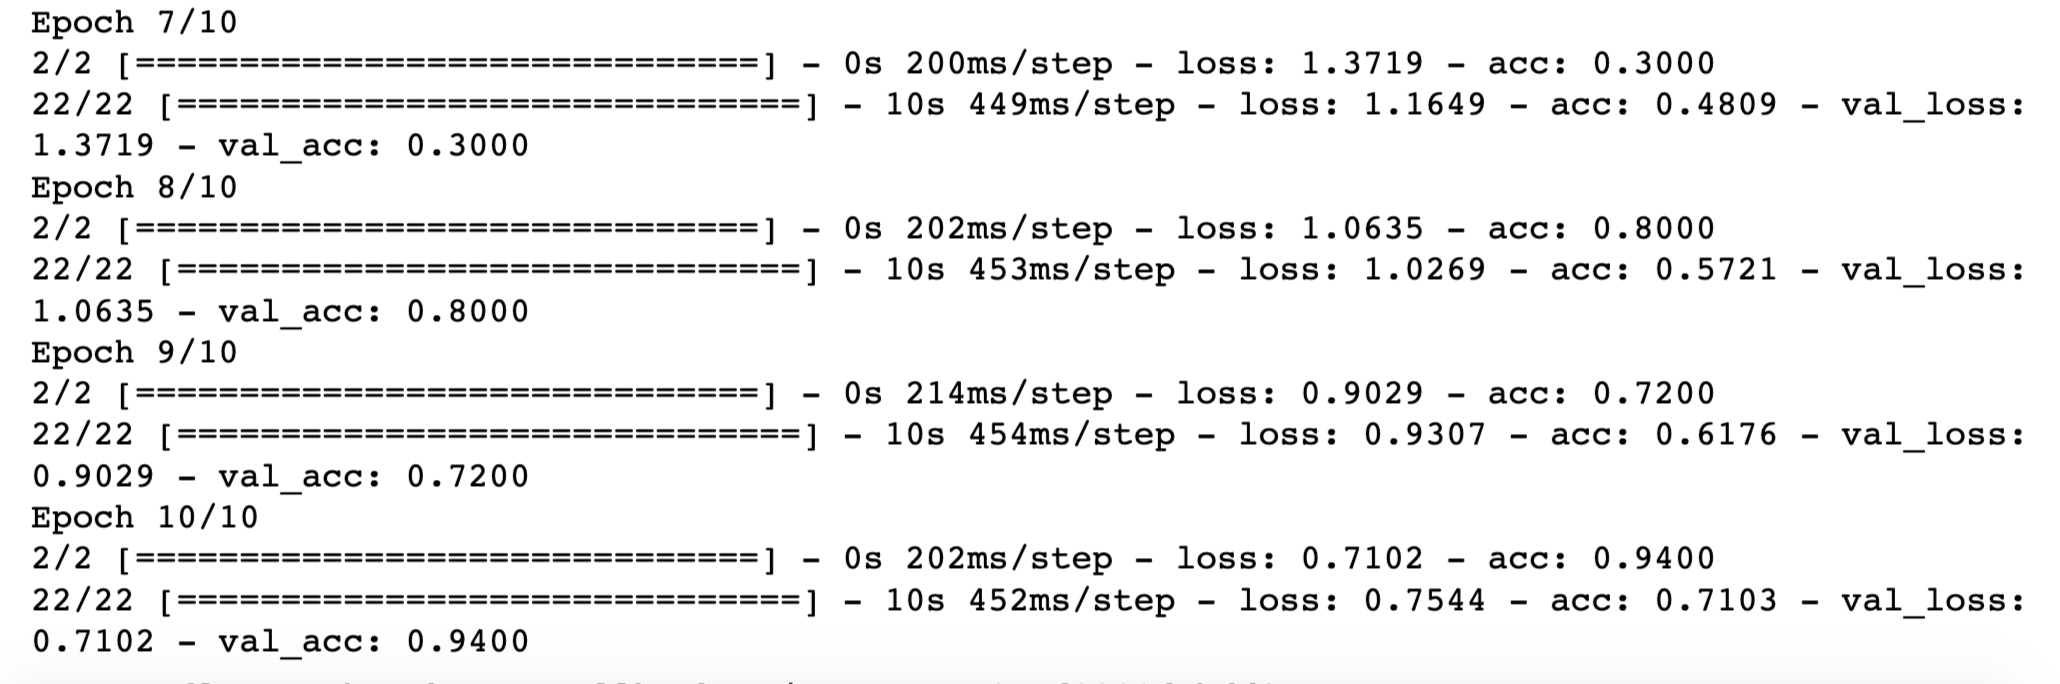
\includegraphics[width=140mm, height=50mm]{results.png}
\end{figure}

I also set aside 50 images as a hold-out test set. The test set was being used to make predictions of the raga. The results below show that the algorithm was able to correctly classify the labels of unseen data. The script for setting up this prediction is shown below as well as results.

\begin{lstlisting}
test_generator.reset()
pred=classifier.predict_generator(test_generator,
steps=STEP_SIZE_TEST,
verbose=1)

pred_bool = (pred >0.5)

predictions=[]
labels = train_generator.class_indices
labels = dict((v,k) for k,v in labels.items())
for row in pred_bool:
  l=[]
  for index,cls in enumerate(row):
      if cls:
          l.append(labels[index])
  predictions.append(",".join(l))
filenames=test_generator.filenames
results=pd.DataFrame({"file_name":filenames,
                    "predictions":predictions})
\end{lstlisting}

\begin{figure}
  \caption{Sample Prediction Table}
  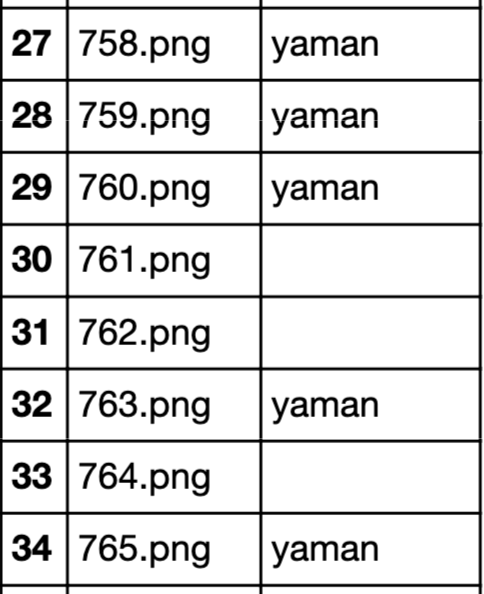
\includegraphics[width=100mm]{pred-table.png}
\end{figure}

As seen in the figure above, the CNN did not output predictions for all the samples in the test set. The reason for this is due to the pred\_bool function which has its bound specified at being greater than 0.5, but this bound is not necessarily the best number to do for multi-class classification problems.
\par
In the final chapter, I talk about my reflection on ways to improve the machine learning analysis as well as future steps for moving from a proof of concept into an intelligent raaga classification software that can be deployed into mobile applications as a tool for musicologists and composers.


\chapter*{\centering Future Steps}
\doublespacing
\setlength{\parindent}{1cm}


\chapter*{\centering Bibliography}
\doublespacing
\setlength{\parindent}{1cm}


\chapter*{\centering Appendix}
\appendix


\end{document}
